\documentclass[tikz,border=12pt]{standalone}
\usepackage[utf8]{inputenc}
\usepackage[T1]{fontenc}
\usepackage{lmodern}
\usepackage{array}
\usepackage{tikz}
\usetikzlibrary{arrows.meta,calc}
\definecolor{greenFill}{HTML}{E8F5E9}
\definecolor{greenStroke}{HTML}{43A047}
\definecolor{coreFill}{HTML}{E1F5FE}
\definecolor{coreStroke}{HTML}{0277BD}
\newcommand{\classcontent}[2]{\begin{tabular}{p{5.8cm}}\centering\bfseries #1\tabularnewline\hline\raggedright\arraybackslash #2\end{tabular}}
\begin{document}
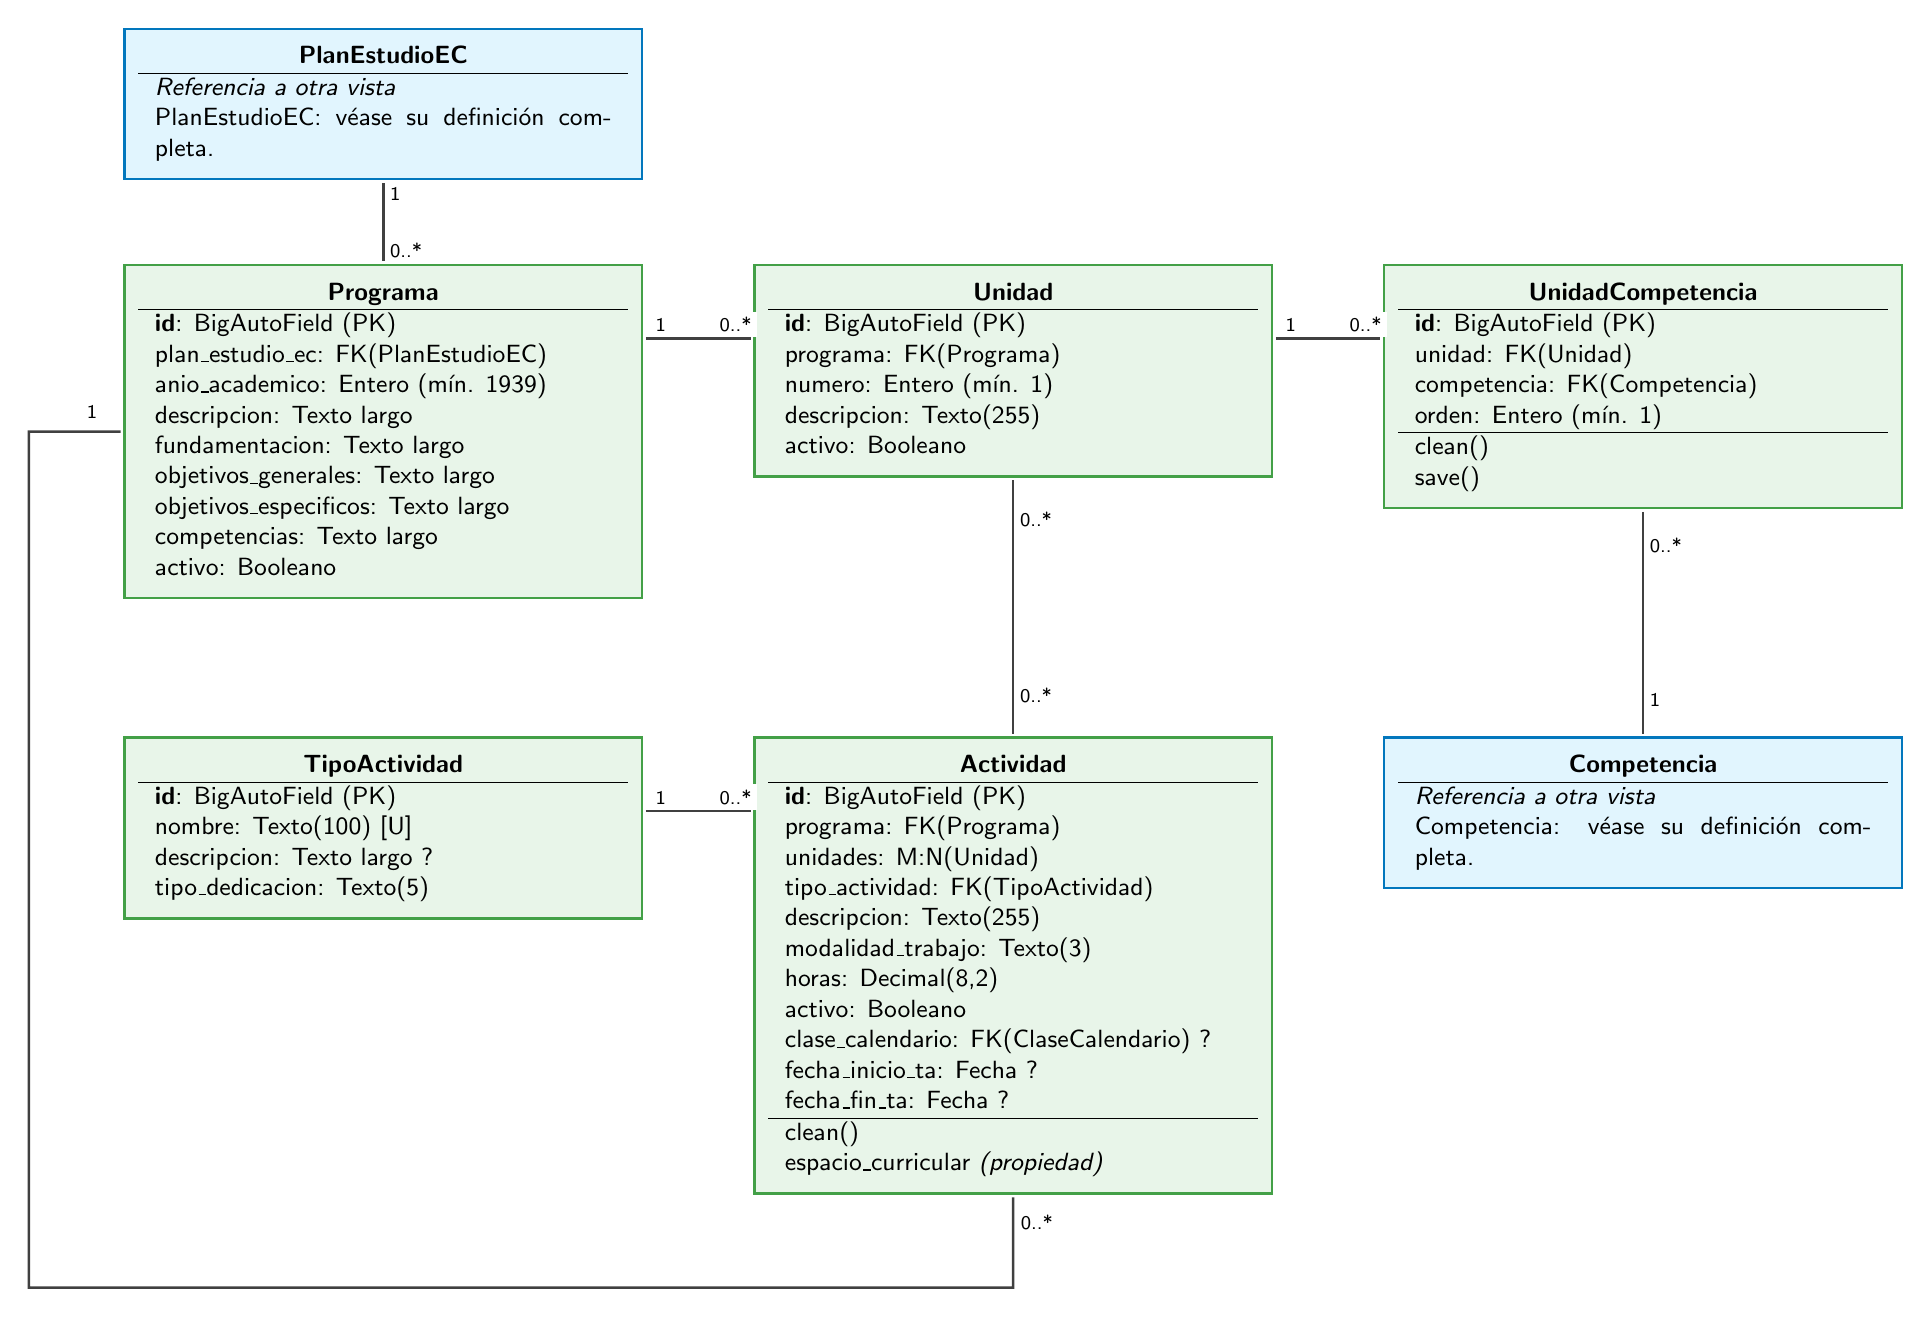
\begin{tikzpicture}[
 font=\sffamily\small,
 cls/.style={rectangle,draw=greenStroke,fill=greenFill,line width=.8pt,inner sep=5pt,anchor=north},
 ref/.style={cls,draw=coreStroke,fill=coreFill},
 association/.style={line width=.9pt,draw=black!75,shorten >=1pt,shorten <=1pt},
 dependency/.style={association,dashed,-{Stealth[length=3mm,width=2.2mm]}},
 mult/.style={font=\sffamily\scriptsize,fill=white,inner sep=2pt,text=black}
]
\node[cls] (Programa) at (0,0) {\classcontent{Programa}{\textbf{id}: BigAutoField (PK)\\plan\_estudio\_ec: FK(PlanEstudioEC)\\anio\_academico: Entero (mín. 1939)\\descripcion: Texto largo\\fundamentacion: Texto largo\\objetivos\_generales: Texto largo\\objetivos\_especificos: Texto largo\\competencias: Texto largo\\activo: Booleano}};
\node[cls] (Unidad) at (8,0) {\classcontent{Unidad}{\textbf{id}: BigAutoField (PK)\\programa: FK(Programa)\\numero: Entero (mín. 1)\\descripcion: Texto(255)\\activo: Booleano}};
\node[cls] (UnidadCompetencia) at (16,0) {\classcontent{UnidadCompetencia}{\textbf{id}: BigAutoField (PK)\\unidad: FK(Unidad)\\competencia: FK(Competencia)\\orden: Entero (mín. 1)\\\hline clean()\\save()}};
\node[cls] (TipoActividad) at (0,-6) {\classcontent{TipoActividad}{\textbf{id}: BigAutoField (PK)\\nombre: Texto(100) [U]\\descripcion: Texto largo ?\\tipo\_dedicacion: Texto(5)}};
\node[cls] (Actividad) at (8,-6) {\classcontent{Actividad}{\textbf{id}: BigAutoField (PK)\\programa: FK(Programa)\\unidades: M:N(Unidad)\\tipo\_actividad: FK(TipoActividad)\\descripcion: Texto(255)\\modalidad\_trabajo: Texto(3)\\horas: Decimal(8,2)\\activo: Booleano\\clase\_calendario: FK(ClaseCalendario) ?\\fecha\_inicio\_ta: Fecha ?\\fecha\_fin\_ta: Fecha ?\\\hline clean()\\espacio\_curricular \textit{(propiedad)}}};
\node[ref] (Competencia) at (16,-6) {\classcontent{Competencia}{\textit{Referencia a otra vista}\\Competencia: véase su definición completa.}};
\draw[association] ($(Programa.north east)+(0,-.95)$) -- ($(Unidad.north west)+(0,-.95)$) node[pos=.16,above,mult]{1} node[pos=.84,above,mult]{0..*};
\draw[association] ($(Unidad.north east)+(0,-.95)$) -- ($(UnidadCompetencia.north west)+(0,-.95)$) node[pos=.16,above,mult]{1} node[pos=.84,above,mult]{0..*};
\draw[association] (UnidadCompetencia.south) -- (Competencia.north) node[pos=.16,right,mult]{0..*} node[pos=.84,right,mult]{1};
\draw[association] ($(TipoActividad.north east)+(0,-.95)$) -- ($(Actividad.north west)+(0,-.95)$) node[pos=.16,above,mult]{1} node[pos=.84,above,mult]{0..*};
\draw[association] (Unidad.south) -- (Actividad.north) node[pos=.16,right,mult]{0..*} node[pos=.84,right,mult]{0..*};
\draw[association] (Programa.west) -- ($(Programa.west)+(-1.2,0)$) -- (-4.5,-13) -- (8,-13) -- (Actividad.south);
\node[mult] at ($(Programa.west)+(-.4,.25)$) {1};
\node[mult] at ($(Actividad.south)+(.3,-.35)$) {0..*};
\node[ref] (PlanEstudioEC) at (0,3) {\classcontent{PlanEstudioEC}{\textit{Referencia a otra vista}\\PlanEstudioEC: véase su definición completa.}};
\draw[association] (PlanEstudioEC.south) -- (Programa.north) node[pos=.16,right,mult]{1} node[pos=.84,right,mult]{0..*};
\end{tikzpicture}
\end{document}
